\documentclass[tikz,border=5pt]{standalone}
\usepackage{amsmath}
\usetikzlibrary{arrows.meta,calc}
\tikzset{wire/.style={blue!65!black,line width=1.15pt},back/.style={blue!35!black,dashed,thin},
vec/.style={-{Stealth[length=2.2mm]},thick},axis/.style={-{Stealth[length=1.8mm]},thin},
force/.style={-{Stealth[length=2.4mm]},very thick,red!70!black}}
\begin{document}

% statement-04: true horizontal circle and five-turn 3D helix, not stacked disconnected ellipses.
% Both coil endpoints reach the supply circuit; the ring does not connect electrically to it.
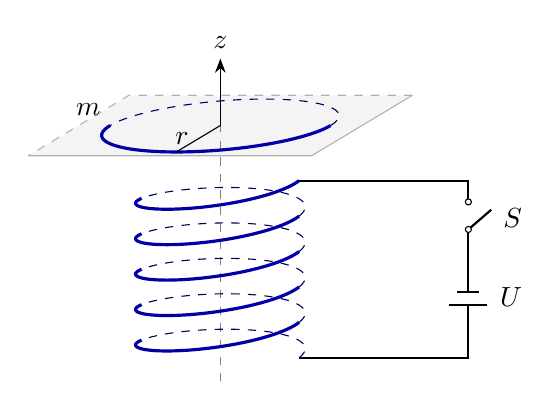
\begin{tikzpicture}[x={(1cm,0cm)},y={(.40cm,.24cm)},z={(0cm,1cm)}]
\fill[gray!9] (-1.8,-1.6,3.1)--(1.8,-1.6,3.1)--(1.8,1.6,3.1)--(-1.8,1.6,3.1)--cycle;
\draw[gray!60,thin] (-1.8,-1.6,3.1)--(1.8,-1.6,3.1)--(1.8,1.6,3.1);
\draw[gray!60,dashed,thin] (1.8,1.6,3.1)--(-1.8,1.6,3.1)--(-1.8,-1.6,3.1);
\draw[gray,dashed] (0,0,-.15)--(0,0,3.62);
\draw[axis] (0,0,3.1)--(0,0,3.95) node[above] {$z$};
\foreach \j in {0,...,4}{
  \draw[back] plot[domain=0:180,samples=45,variable=\p]
    ({cos(\p)},{sin(\p)},{.15+(.45)*(\j+\p/360)});
  \draw[wire] plot[domain=180:360,samples=45,variable=\p]
    ({cos(\p)},{sin(\p)},{.15+(.45)*(\j+\p/360)});
}
\draw[back] plot[domain=0:180,samples=50,variable=\p] ({1.4*cos(\p)},{1.4*sin(\p)},3.1);
\draw[wire] plot[domain=180:360,samples=50,variable=\p] ({1.4*cos(\p)},{1.4*sin(\p)},3.1);
\draw[thin] (0,0,3.1)--(0,-1.4,3.1) node[midway,left] {$r$};
\node[above left] at (-1.4,0,3.1) {$m$};
\draw[thick] (1,0,.15)--(3.15,0,.15)--(3.15,0,.82);
\draw[thick] (1,0,2.4)--(3.15,0,2.4)--(3.15,0,2.13);
\draw[thick] (3.15,0,.99)--(3.15,0,1.78);
\draw[thick] (3.01,0,.99)--(3.29,0,.99);
\draw[thick] (2.91,0,.82)--(3.39,0,.82);
\draw[thick] (3.15,0,1.78)--(3.44,0,2.03);
\filldraw[fill=white] (3.15,0,1.78) circle[radius=1.1pt];
\filldraw[fill=white] (3.15,0,2.13) circle[radius=1.1pt];
\node[right] at (3.47,0,1.92) {$S$};
\node[right] at (3.43,0,.92) {$U$};
\end{tikzpicture}

% element-04: positive I, tangent, radial field and vertical force have the actual cylindrical orientation.
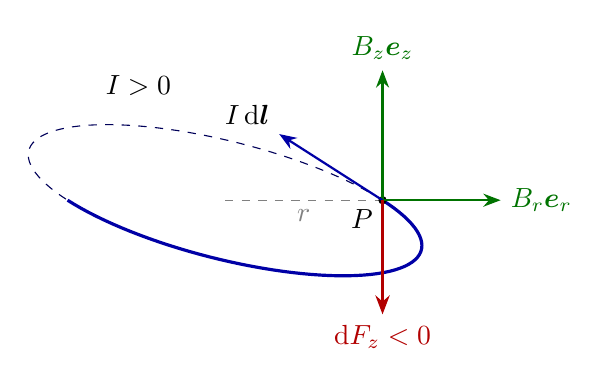
\begin{tikzpicture}[x={(1cm,0cm)},y={(-.75cm,.48cm)},z={(0cm,1cm)}]
\draw[back] plot[domain=0:180,samples=60,variable=\p] ({2*cos(\p)},{2*sin(\p)},0);
\draw[wire] plot[domain=180:360,samples=60,variable=\p] ({2*cos(\p)},{2*sin(\p)},0);
\coordinate (P) at (2,0,0);
\draw[gray,dashed] (0,0,0)--(P) node[midway,below] {$r$};
\fill (P) circle[radius=1.5pt];\node[below left] at (P) {$P$};
\draw[vec,green!45!black] (P)--(3.5,0,0) node[right] {$B_r\boldsymbol e_r$};
\draw[vec,green!45!black] (P)--(2,0,1.65) node[above] {$B_z\boldsymbol e_z$};
\draw[vec,blue!65!black] (P)--(2,1.75,0);
\node[above left] at (2,1.75,0) {$I\,\mathrm d\boldsymbol l$};
\draw[force] (P)--(2,0,-1.45) node[below] {$\mathrm dF_z<0$};
\node at (-1.1,0,1.45) {$I>0$};
\end{tikzpicture}

% flux-04: outward normals, bottom negative flux and positive side flux.
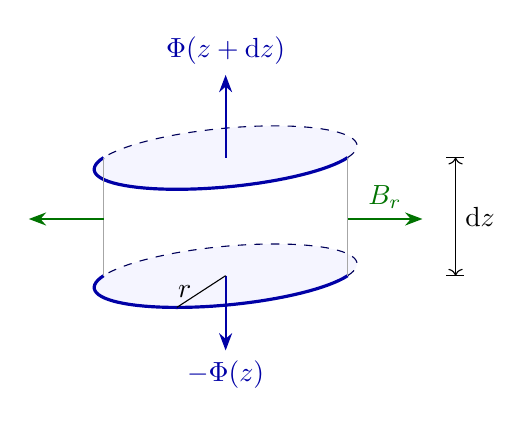
\begin{tikzpicture}[x={(1cm,0cm)},y={(.40cm,.26cm)},z={(0cm,1cm)}]
\foreach \h in {0,1.5}{
  \fill[blue!4] plot[domain=0:360,samples=70,variable=\p] ({1.55*cos(\p)},{1.55*sin(\p)},\h)--cycle;
  \draw[back] plot[domain=0:180,samples=45,variable=\p] ({1.55*cos(\p)},{1.55*sin(\p)},\h);
  \draw[wire] plot[domain=180:360,samples=45,variable=\p] ({1.55*cos(\p)},{1.55*sin(\p)},\h);
}
\draw[gray!70] (-1.55,0,0)--(-1.55,0,1.5);
\draw[gray!70] (1.55,0,0)--(1.55,0,1.5);
\draw[vec,blue!65!black] (0,0,1.5)--(0,0,2.55) node[above] {$\Phi(z+\mathrm dz)$};
\draw[vec,blue!65!black] (0,0,0)--(0,0,-.95) node[below] {$-\Phi(z)$};
\draw[vec,green!45!black] (1.55,0,.72)--(2.5,0,.72) node[midway,above] {$B_r$};
\draw[vec,green!45!black] (-1.55,0,.72)--(-2.5,0,.72);
\draw[thin] (0,0,0)--(0,-1.55,0) node[midway,left] {$r$};
\draw[thin] (2.8,0,0)--(3.03,0,0);\draw[thin] (2.8,0,1.5)--(3.03,0,1.5);
\draw[<->,thin] (2.92,0,0)--(2.92,0,1.5) node[midway,right] {$\mathrm dz$};
\end{tikzpicture}

% motion-04: true horizontal rings shown in perspective; current arrows follow the positive circular parametrization.
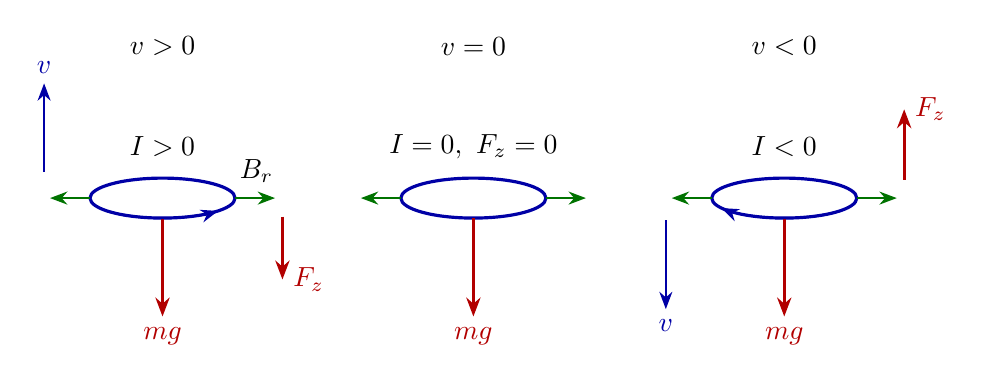
\begin{tikzpicture}[scale=.94]
\foreach \j in {0,1,2}{
 \begin{scope}[xshift={4.2*\j cm}]
 \draw[wire] (0,0) ellipse[x radius=.98,y radius=.27];
 \draw[vec,green!45!black] (.98,0)--(1.52,0);
 \draw[vec,green!45!black] (-.98,0)--(-1.52,0);
 \draw[force] (0,-.27)--(0,-1.6) node[below] {$mg$};
 \end{scope}
}
\node at (0,2.05) {$v>0$};
\node[above] at (1.27,.08) {$B_r$};
\draw[vec,blue!65!black] (-1.6,.35)--(-1.6,1.55) node[above] {$v$};
\draw[force] (1.62,-.25)--(1.62,-1.10) node[right] {$F_z$};
\draw[vec,blue!65!black] plot[domain=210:320,samples=35,variable=\p] ({.98*cos(\p)},{.27*sin(\p)});
\node at (0,.70) {$I>0$};
\node at (4.2,2.05) {$v=0$};\node at (4.2,.70) {$I=0,\ F_z=0$};
\node at (8.4,2.05) {$v<0$};
\draw[vec,blue!65!black] (6.8,-.3)--(6.8,-1.5) node[below] {$v$};
\draw[force] (10.02,.25)--(10.02,1.2) node[right] {$F_z$};
\draw[vec,blue!65!black] plot[domain=320:210,samples=35,variable=\p] ({8.4+.98*cos(\p)},{.27*sin(\p)});
\node at (8.4,.70) {$I<0$};
\end{tikzpicture}

% graphs-04: illustrative eta=1 only; u*=ln2; positive return u=1.59362426004.
\begin{tikzpicture}[scale=1.03]
\def\us{.693147180559945}\def\ur{1.59362426004004}
\begin{scope}
 \draw[axis] (-.15,0)--(5.25,0) node[right] {$u$};
 \draw[axis] (0,-1.96)--(0,2.15) node[above] {$v/(g\tau)$};
 \draw[gray,dashed] (0,-1.7)--(4.84,-1.7);\node[left] at (0,-1.7) {$-1$};
 \node[left] at (0,1.7) {$1$};
 \draw[wire] plot[domain=0:2.2,samples=100,variable=\u] ({2.2*\u},{1.7*(2*exp(-\u)-1)});
 \draw[gray,dashed] ({2.2*\us},1.7)--({2.2*\us},-.53);
 \fill ({2.2*\us},0) circle[radius=1.4pt];\node[below left] at ({2.2*\us},-.54) {$u_*$};
 \node at (3.30,1.50) {$\eta=1$};
\end{scope}
\begin{scope}[xshift=7.0cm]
 \draw[axis] (-.15,0)--(5.25,0) node[right] {$u$};
 \draw[axis] (0,-1.72)--(0,1.90) node[above] {$z/(g\tau^2)$};
 \draw[wire] plot[domain=0:2.2,samples=100,variable=\u] ({2.2*\u},{3.3*(2*(1-exp(-\u))-\u)});
 \draw[gray,dashed] ({2.2*\us},0)--({2.2*\us},{3.3*(1-\us)});
 \fill ({2.2*\us},{3.3*(1-\us)}) circle[radius=1.4pt];
 \node[above] at ({2.2*\us},{3.3*(1-\us)}) {$1-\ln2$};
 \node[below] at ({2.2*\us},0) {$u_*$};
 \fill ({2.2*\ur},0) circle[radius=1.4pt];\node[above right] at ({2.2*\ur},0) {$u_{\mathrm{ret}}$};
 \node at (3.80,1.45) {$\eta=1$};
\end{scope}
\end{tikzpicture}
\end{document}
